%
% pie.tex
%
\section{Chart::Pie}
\name{Chart::Pie}
\file{Pie.pm}
\requires{Chart::Base, GD, Carp, FileHandle}
\begin{Description} 
\class{Pie} is a subclass of class \class{Chart::Base}.
The class \class{Pie} creates a pie chart. The first added set are the labels. 
The second set are the values.
\end{Description}

\parindent 0pt{\large Example:}

\begin{figure}[h]
	\begin{center}
		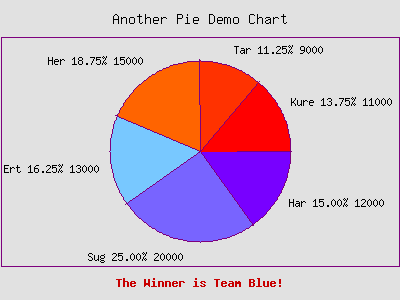
\includegraphics[scale = 0.6]{d_pie3.png}
	\end{center}
	\caption{Pie chart}
	\label{fig:pie}
\end{figure}
\begin{verbatim}
use Chart::Pie;

$g = Chart::Pie->new();

$g->add_dataset ('Har', 'Sug', 'Ert', 'Her', 'Tar', 'Kure');
$g->add_dataset (12000, 20000 , 13000, 15000, 9000, 11000  );

%opt = ( 'title' => 'Another Pie Demo Chart',
         'label_values' => 'both',
         'legend' => 'none',
         'text_space' => 10,
         'png_border' => 1,
         'graph_border' => 0,
         'colors' => { 'x_label' => 'red',
                       'misc' => 'plum',
                       'background' => 'grey',
                       'dataset0' => [120, 0, 255],
                       'dataset1' => [120, 100, 255],
                       'dataset2' => [120, 200, 255],
                       'dataset3' => [255, 100, 0],
                       'dataset4' => [255, 50, 0],
                       'dataset5' => [255, 0, 0],
                     },
         'x_label' => 'The Winner is Team Blue!',
        );

$g->set (%opt);

$g->png ("pie.png");
\end{verbatim}

\begin{Constructor} 
An instance of a pie chart object can be created with the constructor \textit{new()}:
\begin{quote}
\fett{\$obj = Chart::Pie->new();}\\
\fett{\$obj = Chart::Pie->new(\parameter{width}, \parameter{height});}
\end{quote}

If \textit{new()} has no arguments, 
the constructor returns an image with the size 300x400 pixels. 
If \textit{new()} has two arguments \parameter{width} and \parameter{height}, 
it returns an image within the desired size.
\end{Constructor}

\Methods
All universal valid methods, see page \pageref{methods} of class \class{Chart::Base}.\\[\parabstand]
%
\Attributes
All universal valid options, see page \pageref{options}. 
Also available, these special options:
\begin{description}
\item['label\_values'] 
          Tells the pie chart what labels to draw beside the pie. 
          Valid values are 'percent', 'value', 'both' and 'none'. Defaults to 'percent'.

\item['legend\_label\_values'] 
          Tells the pie chart what labels to draw in the legend. 
          Valid values are 'percent', 'value', 'both' and 'none'. Defaults to 'value'.
          
\item['legend\_lines']
          The labels drawn aside the pie are connected with a line to the segment.
          
\item['ring']
          The pie has a ring structure.          

\end{description}
